\documentclass[bsc,frontabs,twoside,singlespacing,parskip]{infthesis} 
\usepackage{graphicx}
\usepackage{listings}
\usepackage{url}
\usepackage{xfrac} 
\graphicspath{ {images/} }

\begin{document}

\title{Text Driven Talking Heads}

\author{Iain Brown}
\course{Computer Science}
\project{Undergraduate Dissertation} 
%\project{Undergraduate Thesis} % AI%Psy
%\project{4th Year Project Report}

\date{\today}
%\abstract{The aim of this project is to build a head motion synthesizer for a lifelike animated avatar. The head motions will be predicted entirely from the text of transcribed speech with the aim of finding a mapping between the text and natural head motions. Unlike previous areas of research where the head motions are generated from recorded speech.}
\maketitle
%\section*{Acknowledgements}
%Acknowledgements go here. 
\tableofcontents

% ============================================================= %
\chapter{Introduction}

%The Introduction chapter should always provide a 'roadmap' to the report. Of course it should provide an introduction to the problem being considered, but it should also give some details of what you did - do not leave this to the conclusion. You should give forward references into the rest of the report - e.g., "In Chapter 2 how algorithms and heuristics are used to deal with approximate counting are discussed", "The design of the system is presented in Chapter 4", "In Chapter 3 the reasons for choosing to focus on the bounded-degree case of this problem are explained"
%

- Head motion is very important when it comes to human communication \\
- Dialogue is much harder to fully understand without the non-verbal information \\
- Generating Lifelike avatars in many applications, VR, video games, shopping assistant \\
- Realistic head motions are vital otherwise humans may feel weird interacting with an avatar \\
- Project aimed to create a system that synthesises natural head motions just from the text \\
- Without knowledge present in speech \\
- Using Various Natural Language Processing Techniques \\

% ============================================================= %
\chapter{Background Information}

\section{Human Computer Interaction}

Human Computer Interaction is a field of Computer Science in constant change. With the goal of enhancing Human Computer Interaction researchers have looked to the field of Embodied Conversational Agents, where an intelligent agent is mapped to a graphical animation or body to replicate the most natural of interactions: face to face dialogue. \cite{ecas} 

Embodied Conversational Agents have had been found to enhance the interactions with computers \cite{conv_agents} and researchers are perpetually improving systems in order to increase user satisfaction. One of the biggest benefits to using an ECA is that the interaction is of a social nature, being more familiar to humans and aids the systems perceived trust worthiness, allowing a richer interaction between the user and the computer. Also the intelligibility of speech produced in noise is also improved when a speaker's face is visible \cite{emotion_head_motion}, this means that because the user has a physical representation of the ECA they can more easily understand what the agent is saying rather than if it was just speech output. These results suggest that nonverbal gestures such as head movements play a more direct role in the perception of speech than previously known. \cite{vis_prosody}

There are some limitations to consider when talking about ECA's, mainly to do with what Masahiro Mori called the Uncanny Valley effect. Mori states that the familiarity with a robot or graphic representation of an avatar increases in correlation with the rise of human likeliness, but there is a distinct fall in familiarity before achieving a life-like human representation referred to as the Uncanny Valley which causes revulsion in humans. \cite{uncanny}

\begin{figure}[h!]
	\centering
	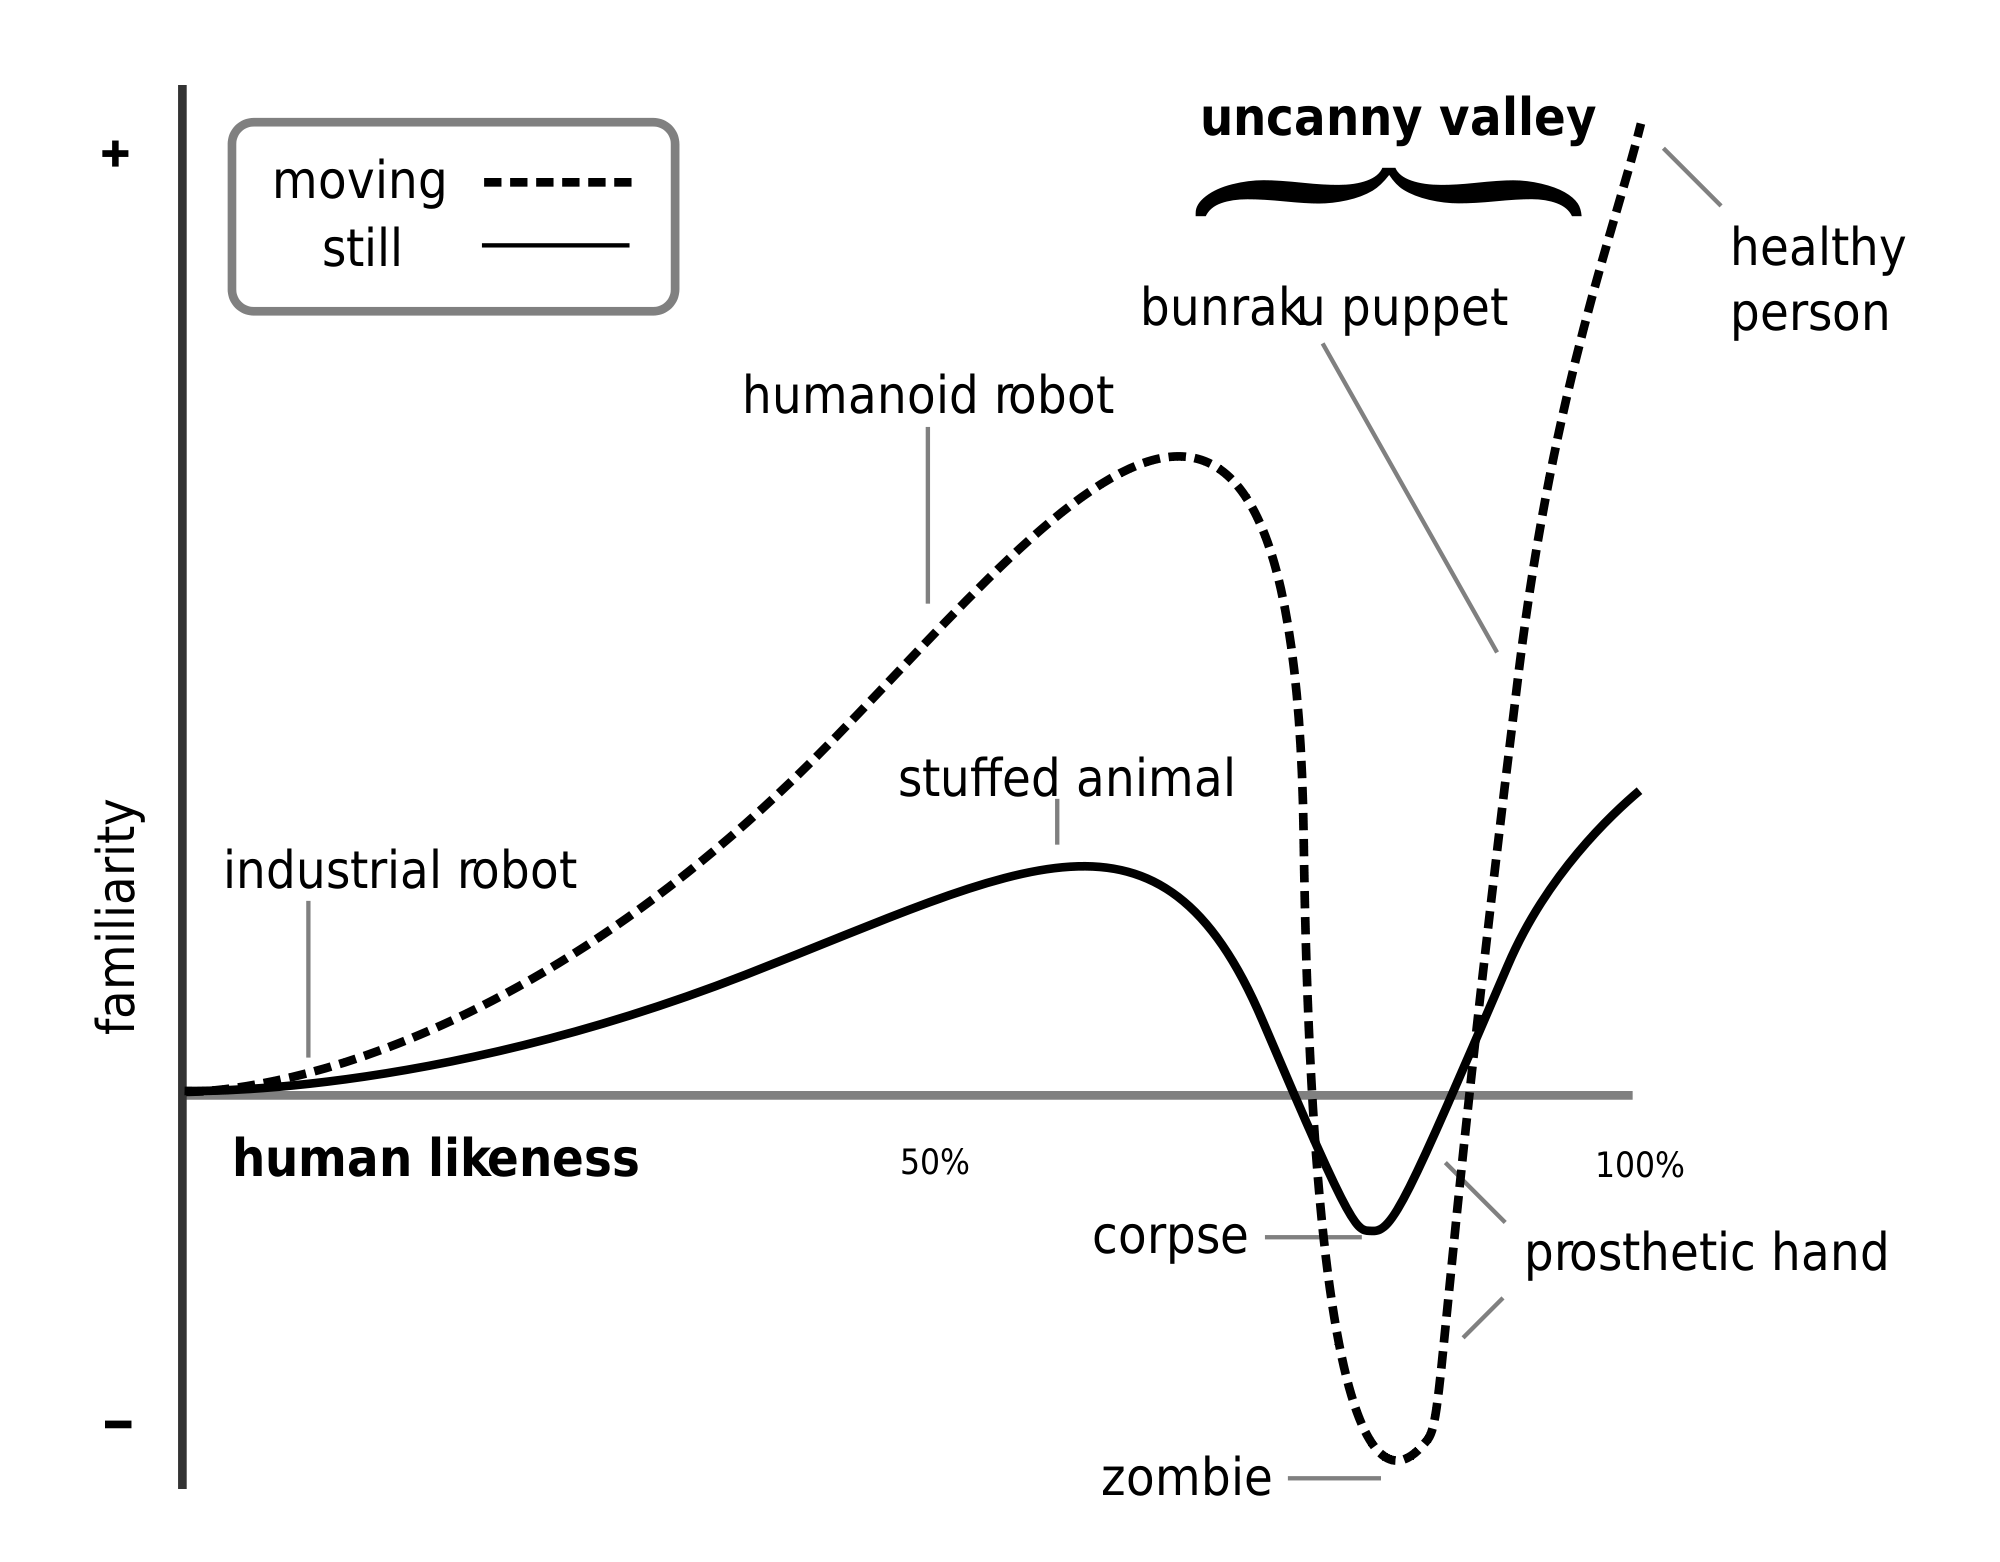
\includegraphics[width=0.6\textwidth]{uncanny}
	\caption{The Uncanny Valley effect}
\end{figure}

\section{Data and Task}

The task for the project was as follows: Using only text transcriptions of speech can we synthesise life-like head motions that seem realistic and natural to humans. The project aimed to investigate the correlation between head motions and the information present in speech unique to the speaker. The difficulty of the task comes from the lack of unique information about the speech, as we are only using the transcribed text. To tackle this we will be using a Text-to-Speech system called Festival.

\subsection{Data Recordings}

The data used for the project was data recordings from the Centre of Speech and Technology Research at Edinburgh University. The recordings consisted of optical motion capture sessions in which participants wore 4 reflective markers on their torso and a hat with 3 reflective markers. There were 7 V100:R2 cameras that tracked the reflective markers at a sampling rate of 100Hz. Participants were asked to read out transcriptions of fairy tales.

\begin{figure}[h!]
	\centering
	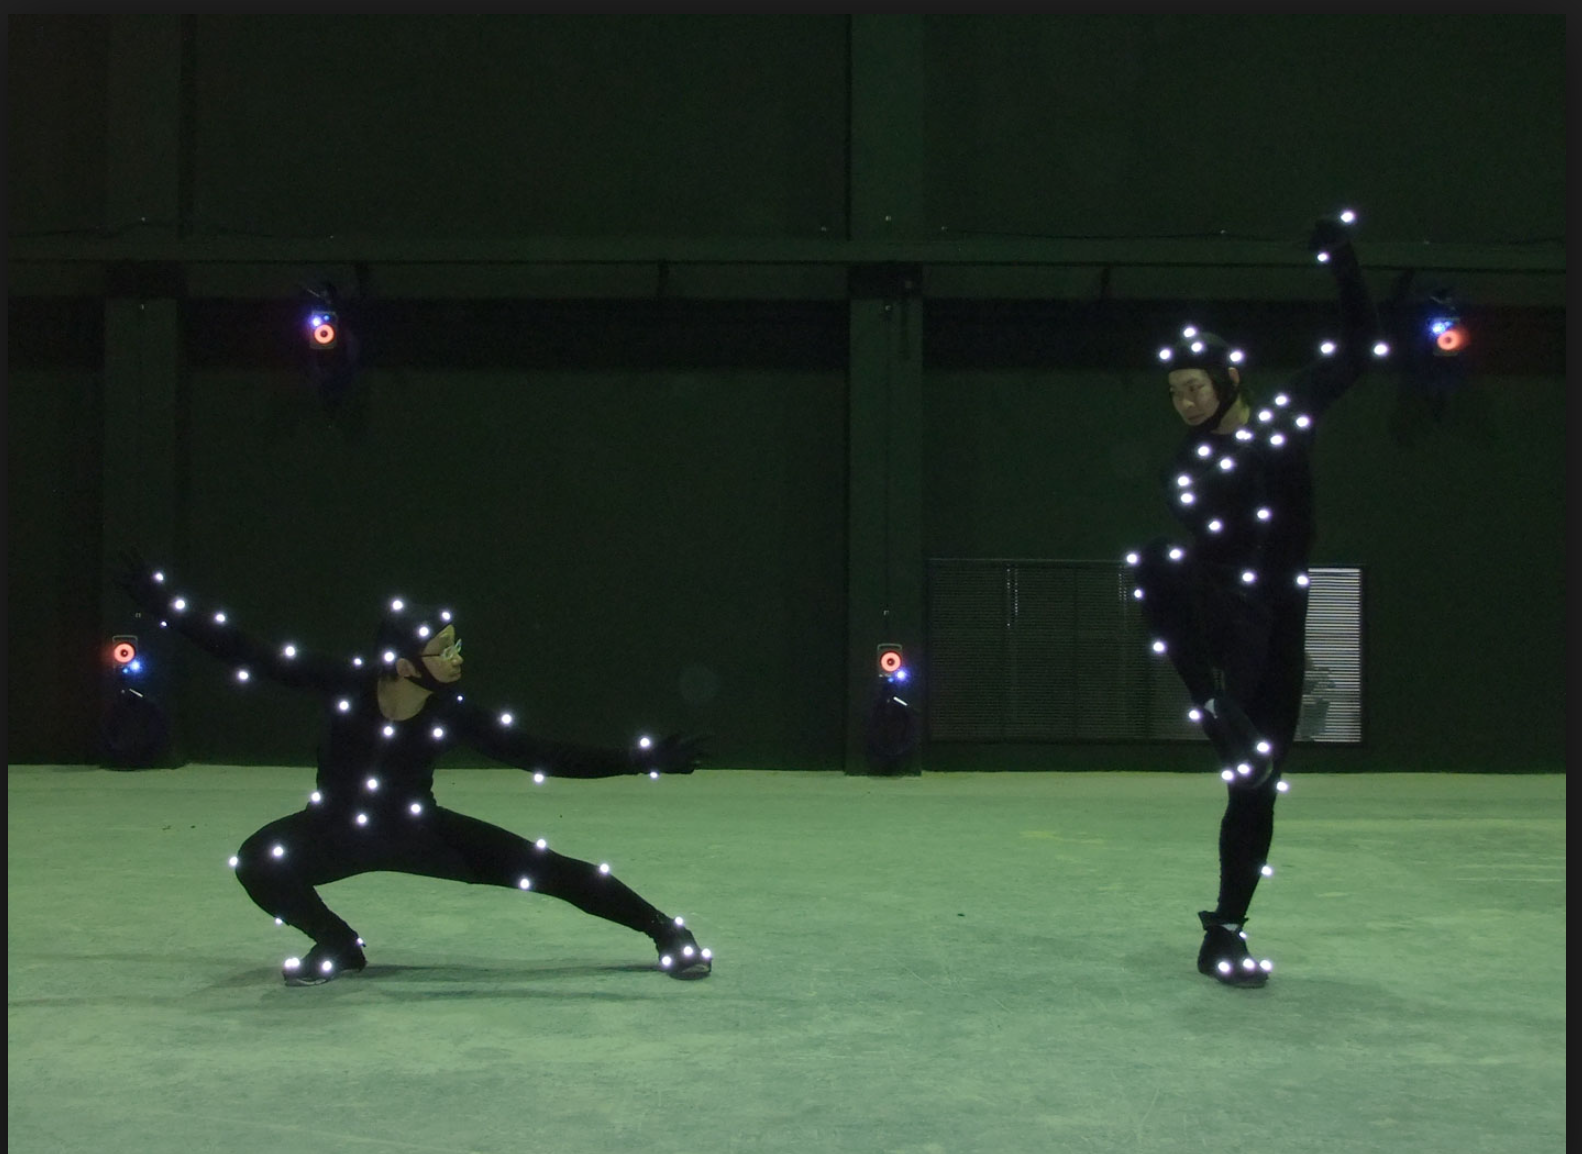
\includegraphics[width=.7\textwidth]{mocap.png}
	\caption{Setup of the mo-cap environment}
\end{figure}

\section{Euler angles}

Euler angles are three angles that represent the orientation of a rigid body in 3-Dimensional space, typically referred to as 'yaw', 'pitch' and 'roll'. Euler angles allows us to reduce the number of parameters normally used to represent rigid body orientation down to 3 parameters. It is a very popular method because of the reduced complexity and is commonly used in robotics and 3D animation software because of this. As the project focused on rigid head motions there was no translation taken into account when designing the 3D avatar head motions. This allowed the project to use Euler angles as the sole units of movement in the project.

\begin{figure}[h!]
	\centering
	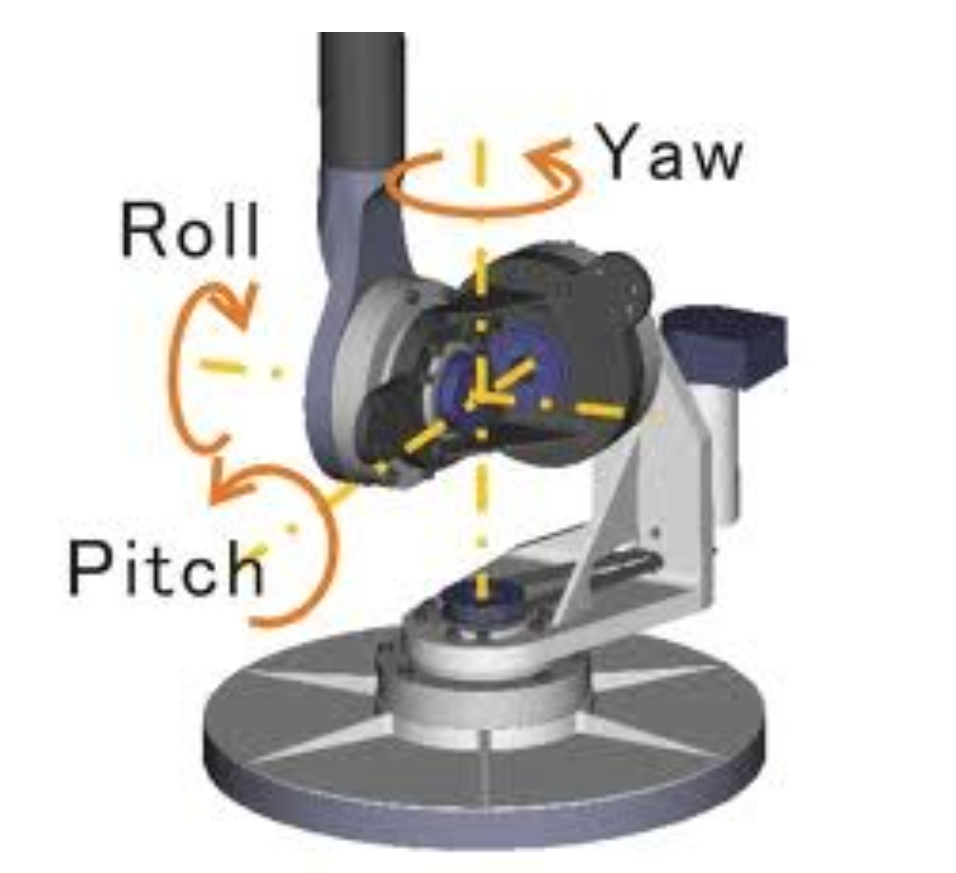
\includegraphics[width=.5\textwidth]{euler_angles.png}
	\caption{Euler Angles in Robotics}
\end{figure}

Euler angles do have some drawbacks. One of the most common issues animators experience with Euler angles is that different results can occur depending on the order of rotation. For example the rotation Roll x Yaw x Pitch will most likely have a completely different effect to the rotation Pitch x Yaw x Roll. \cite{quartionions} Another potential issue is the Gimbal Lock \cite{gimbal}. Euler angles were chosen because of their ease of use and these drawbacks were not an issue.

\section{Poser Animation}

3D animation and rendering software was used to visualise the generated head motions. The software used for this purpose was PoserPro 2012 by Smith Micro Software, a 3D animation tool with the emphasis on character creation and animation. PoserPro allows users to animate body parts of 3D characters and change their characteristic like rotation, translation and scale, meaning that the head of a character could be moved independently with ease.

With a scripting plug-in for Python called PoserPython, \cite{poser_python} allowing users to create scripts to manipulate objects and characters in the scene using Python. This was one of the main reasons for choosing PoserPro over other animation and rendering software like Blender. Poser also uses Euler angles as it's unit of rotation.

\begin{figure}
	\centering
		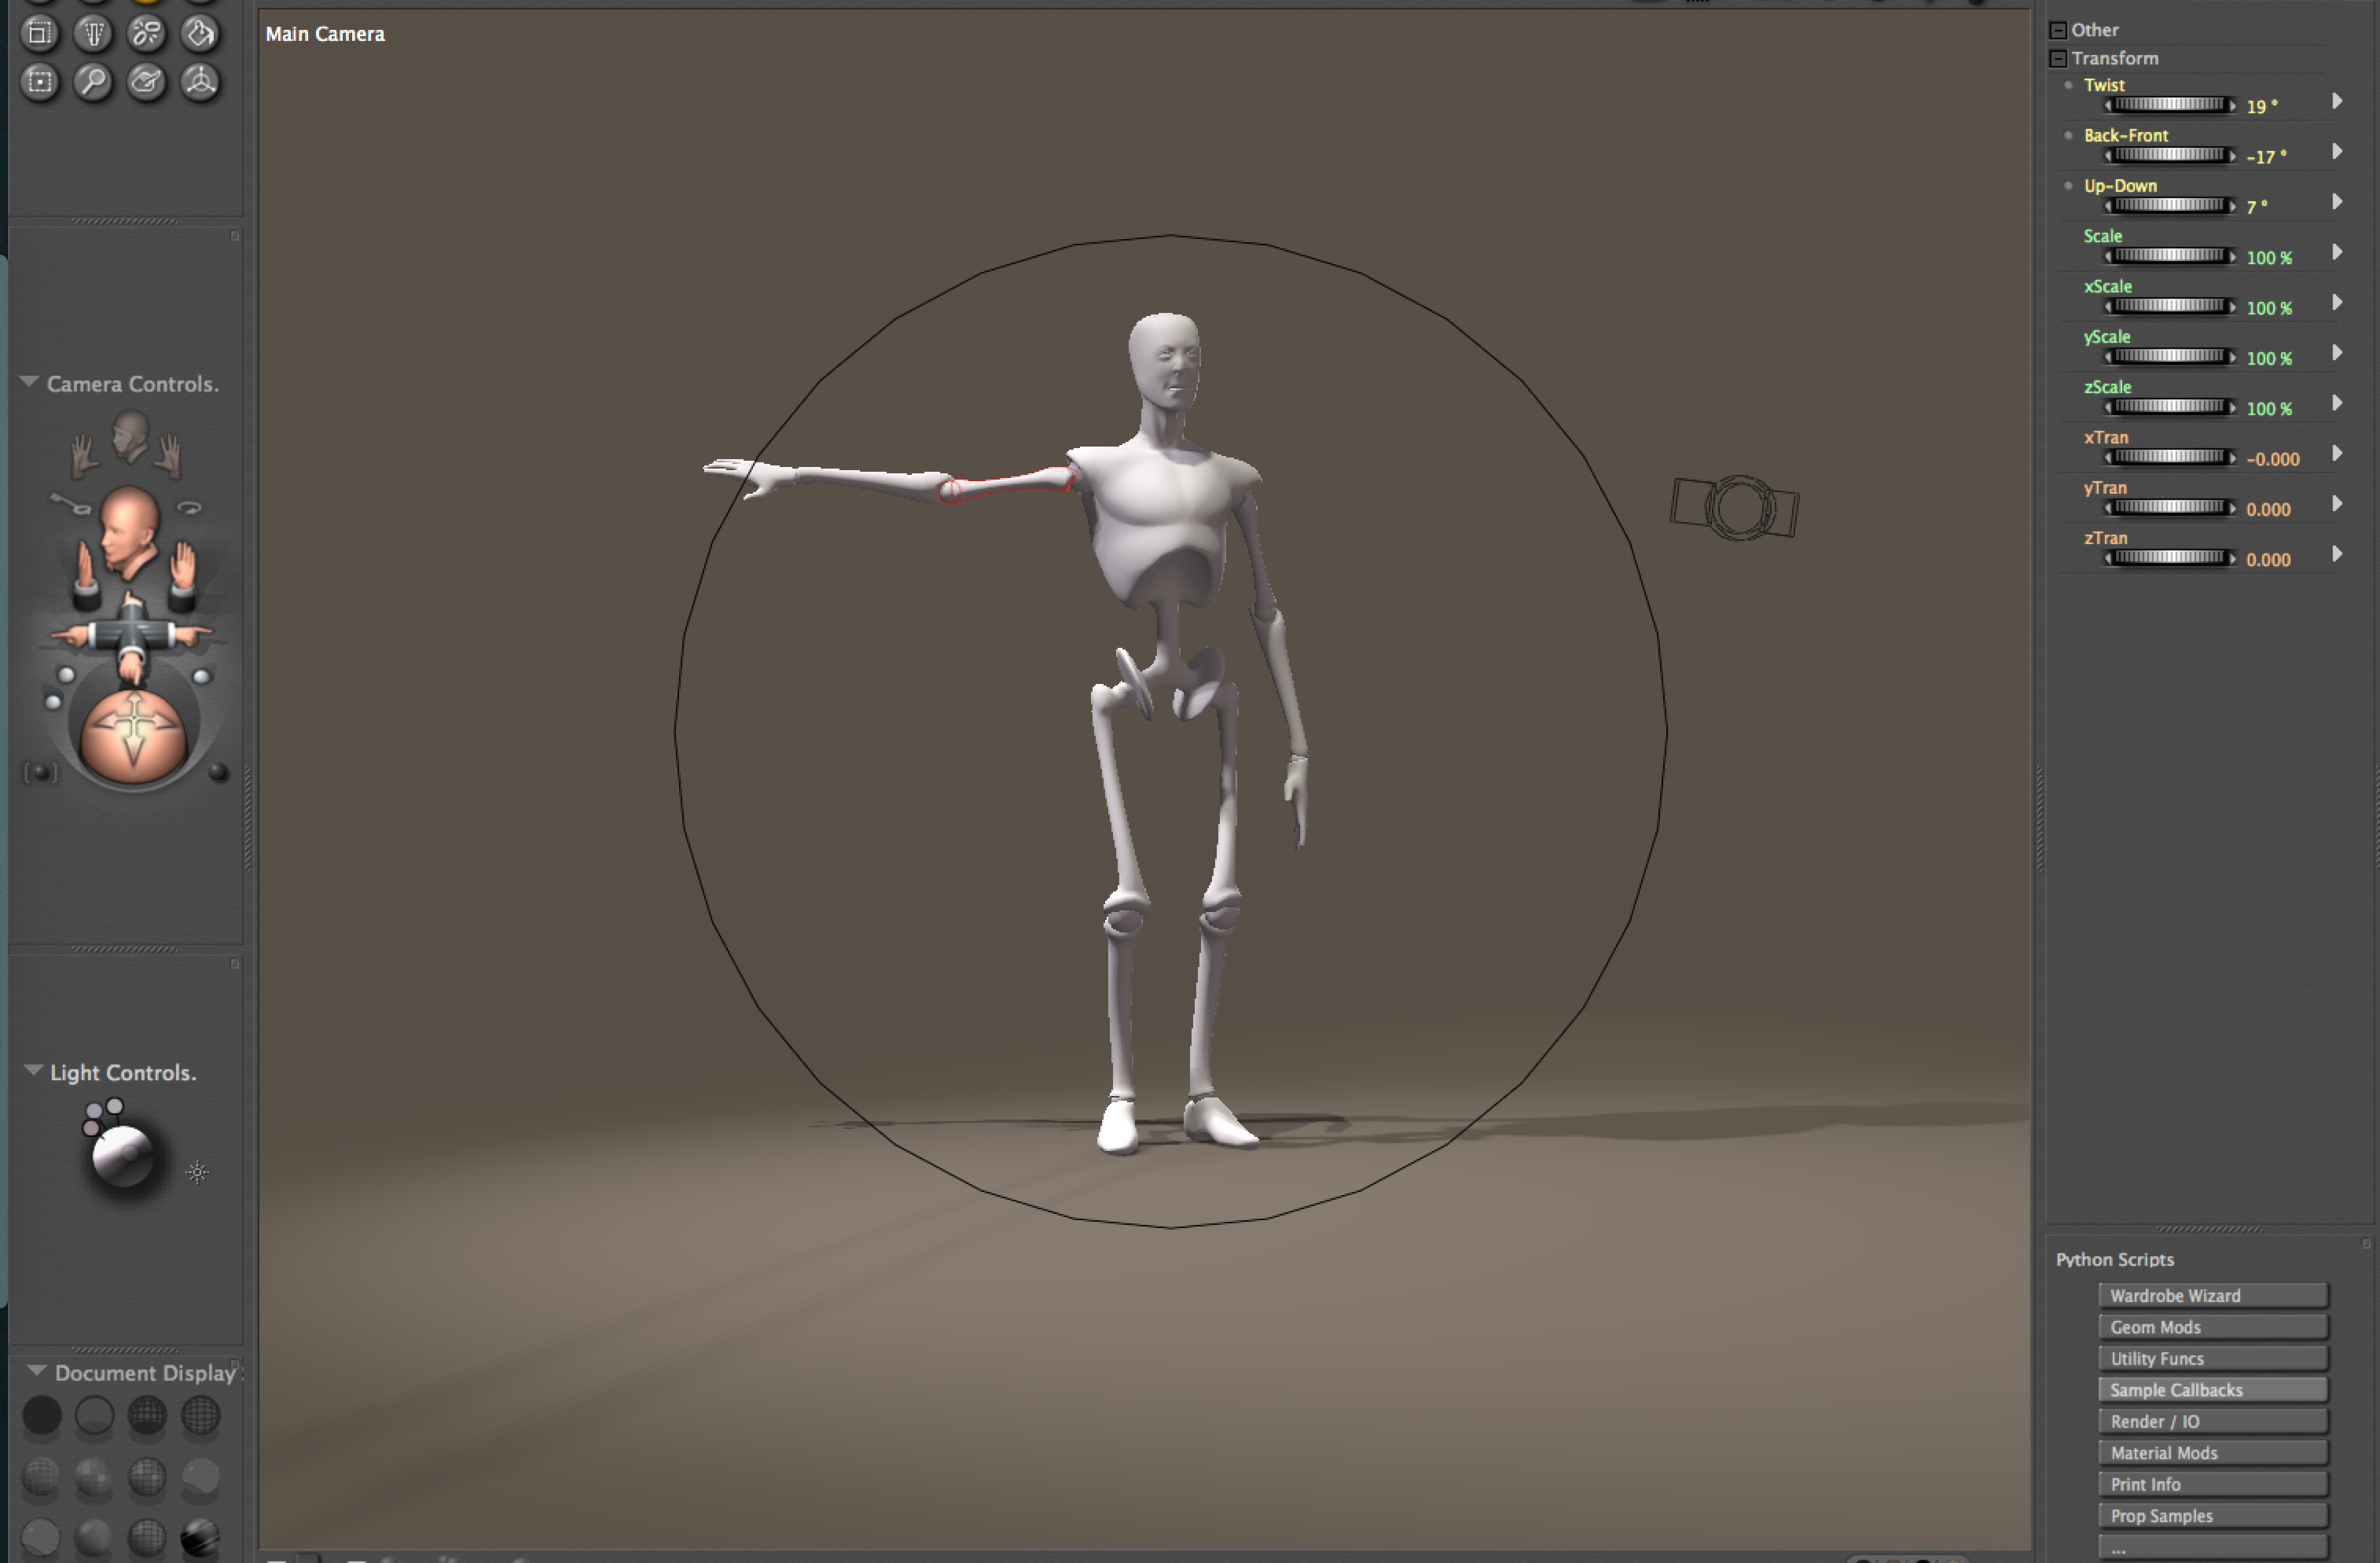
\includegraphics[width=1.0\textwidth]{poser.png}
		\caption{Overview of Poser Pro}
\end{figure}

\section{Facial Animation Approaches}

- Speech Driven Head Motion Synthesis \cite{speech_driven_head_motion}\\
- Facial Animation and Head Motions driven by speech acoustics \cite{facial_animation_acoustics}\\
- Expressive Speech - driven facial animation \cite{expressive_speech_animation}\\
- Rigid Head Motion \cite{rigid_head_motion} \\
- Lip motion from text \cite{lip_motion}

\section{Subjective Evaluation Approaches}

\subsection{Mean Opinion Score - MOS}
\cite{mos}
\subsection{Preference Test}
\subsubsection{AB Test}
\subsubsection{ABX Text}

\subsection{Multiple Stimuli with Hidden Reference and Anchor - MUSHRA}

\cite{mushra}

% ============================================================ %

\chapter{Text-Driven Head Motion Synthesis}
% This will be the theoretical implementation details 
% There needs to be a system architechture map somewhere here.

The goal of this project was to develop a system that was capable of synthesising life-like, realistic head motions from transcribed speech. This project aimed to developed a system that was capable of synthesising head motions given just the text. In order to to this hypotheses about the relation of head motion events and speech content were introduced. The system built on these hypotheses, linking them together in order to synthesis the final head motions. Text itself is very limited in information, so in order to have richer input data the transcribed text would be passed through a Text to Speech system which would apply natural language processing techniques in order to synthesise speech. 

\section{Hypotheses}

It was  found that when two people have a conversation, head motions are more prevalent in the dialogue if the two people do not have a close relationship. \cite{first_paper} In dialogue the nod is commonly understood as a gesture of affirmation and agreement. A possible explanation for this effect could be that because there is no pre-existing relationship humans subconsciously overcompensate their head motions as a method of positive reenforcement to aid in building a foundation for this new relationship. In the context of Embodied Conversational Agents the system aimed to synthesise head motions that made the interaction between the user and the ECA as natural as possible in relation to head motions, to incorporate this hypotheses into the system the main head motion should primarily be a nodding motion and head motions should overcompensate similar to an interaction with a new person with the aim of making the interaction feel more like a face to face conversation and provide a  more comfortable experience.

\subsection{Prosodic Features}

Prosody is the rhythm, stress and intonation of speech. As english is the language domain for the project and english is a stress timed language \cite{stress_timed}, prosodic features in speech are very important to the meaning of speech and can change the meaning of the underlying text.

Head motions correlate strongly with prosody present in speech \cite{vis_prosody}. My first hypothesis relates to the rate of change of the fundamental frequency present in the synthesised speech. This is indicated in the Festival output as values around 120 Hz for male voices and 210Hz for female voices \cite{f0_values}. Sudden changes in the frequency should be reflected in head motions. For example in the intonation falls the head should lower accordingly \cite{Kendon}.

\subsection{Phrasing}

Phrasing plays a huge role in how something is said. It has been found that nodding head motions frequently occur at the end of phrases or at strong phrase boundaries, especially if the speaker is confident in what they are saying. \cite{ishi2008}. 

\subsection{Sentiment Analysis}

Sentiment analysis is a popular area of natural language processing. It is often used to gauge reviews for products\cite{sentiment_online} and films\cite{sentiment_films} due to the availability of data and ease of tagging the reviews as either positive or negative.

Sentiment or emotion in speech has various effects on head motions. In a study It was found that the absence of head motion can be easily identified as 'neutral' emotion. \cite{emotion_head_motion} whereas participants in the study found it difficult to differentiate between head motions that were typical of 'happy' and 'sad' emotions. This study shows that emotive analysis on the text should be treated as an 'intensifier' of the underlying head motions derived form other areas of the text rather than altering the head motions to fit an emotion.

\subsection{Text Content}

There are two types of gestures that relate to speech. \cite{lexical_gestures} The first are motor movements which are typically simple, brief, repetitive and have a high correlation with prosodic features. The other type are lexical movements, gestures that help the speaker mentally perform lexical lookups subconsciously. These gestures are very different to motor movements and are much longer, more complex and relate more to the lexical information in the speech. To portray these ideas in this project, unique words that are not common should cause the avatar to tilt their head. This is similar to the theory that eye movements can aid with memory recall. \cite{eye_movements}

\section{Text analysis with Festival}
TALK ABOUT THE INFORMATION USEFUL TO THE PROJECT \\
WHAT DATA TO USE AND WHY\\


Festival applies various Natural Language Processing techniques to the text to generate information  so that it can synthesise speech.  There are many steps in this pipeline, each adding a little bit more information to the text before Festival can then apply signal processing to generate audio. 

The first stage in the Text to Speech pipeline is the text processing. Festival breaks the text up into more suitable units for processing, for example expanding abbreviations. Then Parts-of-Speech tags are assigned to the units, these POS tags indicate what type of word it is and how it relates to the overall structure of the sentence allowing for phrase break prediction.

Phrase break prediction assigns a break strength to each unit, which highlights where the phrases are in the sentences. Phrase break predictors are usually taggers trained on annotated data and are accurate.


Festival generates pronunciations by performing syllabification, breaking the sentences and words into syllables and looking up phonemes in a lexicon to determine their pronunciations. Using this information the system can generate ToBi markers \cite{tobi}, a way of symbolically representing intonation. These symbols are useful as it they are conceptually easy to understand and reduce the number of parameters needed to understand intonation.

Similarly to phrase break predictors, Festival uses duration predictors that have been trained on annotated data using classification and regression trees to produce duration information for each phoneme.

Now that the system has a linguistic specification of the sentence like the phone sequence, phone duration and pitch contour signal processing can be performed to generate the final speech output.

\begin{figure}[h!]
	\centering
	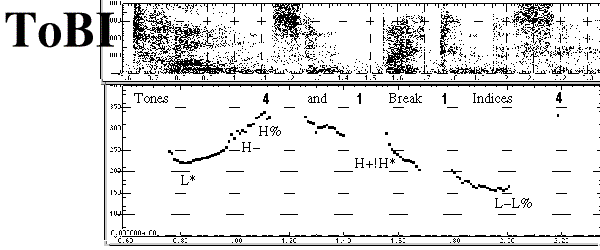
\includegraphics[width=0.8\textwidth]{tobi.png}
	\caption{ToBi Markers}
\end{figure}


\section{Head Motion Synthesis Systems}

\subsection{Basic}

\subsection{Random}

\subsection{Rule Based}

% ============================================================= %
\chapter{Implementation}

The system was implemented using Python, a high-level programming language widely used for many purposes including scripting and large scale software development. Python was the clear choice for many reasons including powerful libraries such as NLTK (Natural Language Toolkit) \cite{nltk} and it's scripting compatibility with Poser. 

The initial difficulty of the project was that there were a lot of individual components to tie together, like Festival and Poser. The subprocess module in Python allows the script to spawn new processes, connect to their input and output and retrieve their return codes. This was invaluable in the project as it allowed the Python script to call Festival with parameters that could change with each run.

\begin{lstlisting}
fest_location = DIR+'preparation/text2utt.sh'
festival = subprocess.Popen(
		[fest_location,text_file], 
		stdout=subprocess.PIPE
		)
utterance = festival.stdout.read()
return utterance
\end{lstlisting}

The data received from the Festival output was a large block of text containing information about the utterance it had processed (See Figure 4.1). This data was fed into a text processing module implemented from scratch to extract the important information regarding the utterance and build a dictionary using these elements to link the individual words with their properties like parts-of-speech tags and phrase break strength.

\begin{figure}
	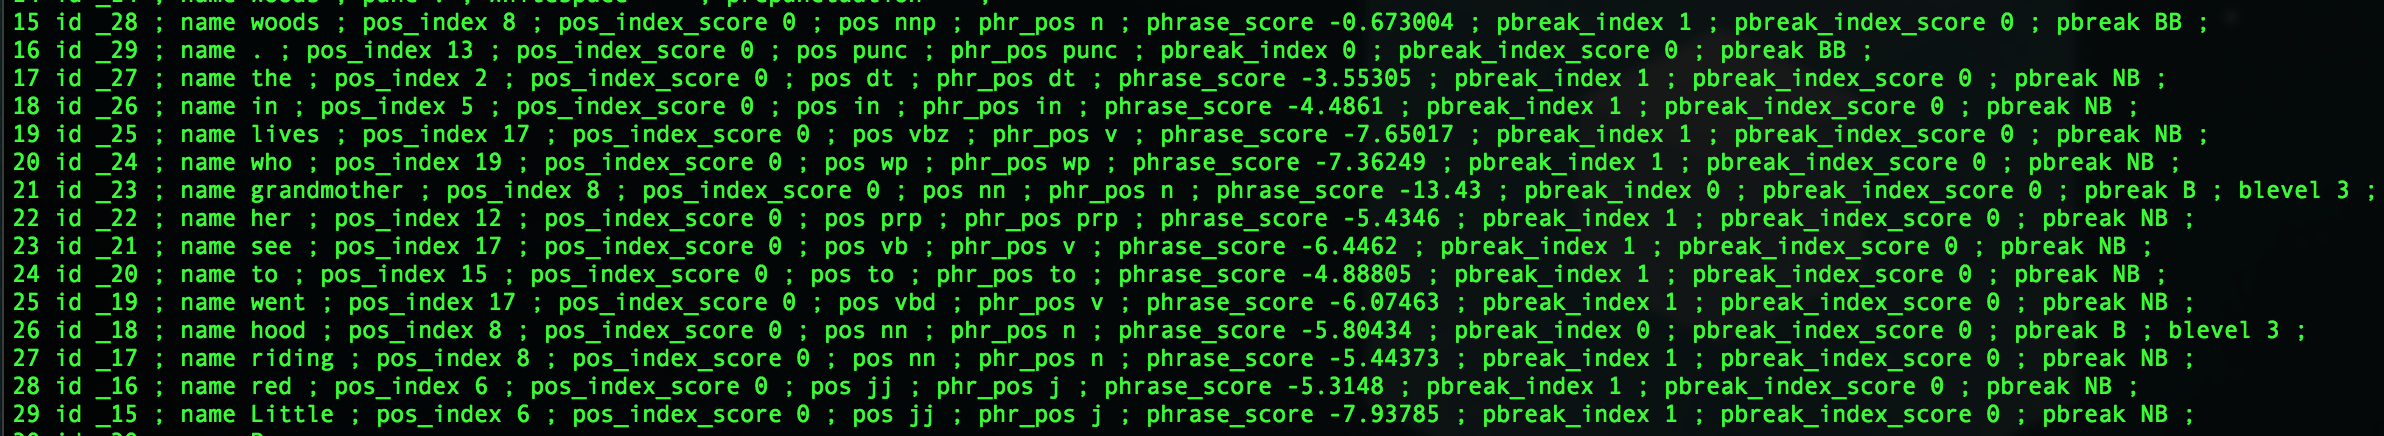
\includegraphics[width=1.0\textwidth]{festival_output.png}
	\caption{An Excerpt from the festival analysis output}
\end{figure}

Normally Festival is run as an interactive interface. The system used a LISP script called "text2utt.sh" that came with the installation, allowing it to run batch commands in "Text to Speech mode" without entering an interactive state. This was perfect for the project but in order to extract duration information correctly and save the outputted speech to audio files the script had to be altered by adding in the following code. 

\begin{lstlisting}
1. (utt.save.words utt outfile 'est_ascii) 
2. (save_waves_during_tts)
\end{lstlisting}

The line of code (save\_waves\_during\_tts) meant that Festival saved all synthesised speech to wave files. An issue that raised from this was that it generated an audio file for each sentence, which was not suitable for the Text-Driven Talking Heads System. This problem was solved by implementing a function in the preparation stage called \"combine\_audio\_files\" which created a new file that was the concatenation of all the sentences. This was a suitable solution as the produced output sounded quite natural.

The Poser Script setMotion.py was taken from another Project that used Euler Angles to rotate a character's limbs, the only alterations made were to set he active body part to the head, add the speech to the scene and to load in the output of the Head Motion Synthesis by hardcoding the name and location of the output file.

The head motion synthesis was developed as three separate modules, increasing in complexity and building on what was successful from the previous head motion synthesis methods.

\section{Basic System} 

NEED TO RESULTS FROM RECORDINGS \\
EXPLAIN THIS WAS SIMILAR TO SINE WAVE \\
EXPALIN WHY CHOICE WAS REASONABLE \\

\subsection{Trignomietric Functions}

As outlined in chapter 3 the most common occurring head motion in dialogue is the nod which was reflected in the analysis of the recorded motion data. This implementation of this hypothesis is the baseline system. It aimed to synthesise a natural nodding motion distributed across the length of the utterance. The nodding motion is a smooth repetitive oscillation of the head along one axis so we represented this using the trigonometric sine function. 

The file basic\_predict.py takes in the dictionary containing all the information retrieved from festival and calculates the number of frames needed for the output rotations and calculates the angle change per frame so that the motion from the first frame to the last frame represents one complete oscillation of the sine formula.

The prediction system adds the rotation information for each Euler angle to the dictionary of utterance data and returns said dictionary. That dictionary is then passed to output.py, which is a generic function that also accepts the utterance dictionary and a filename so that there was no need to re-implement and output function for each system and also allowed for comparison between the systems without necessarily saving them to file allowing rapid prototyping.

%\begin{figure}
%	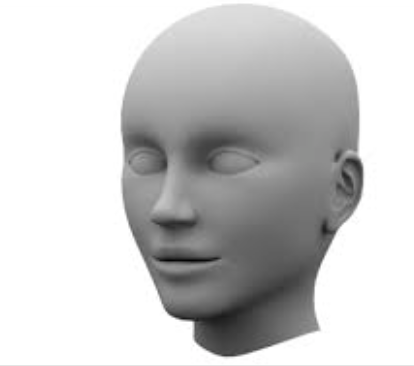
\includegraphics[width=0.3\textwidth]{head.png}
%	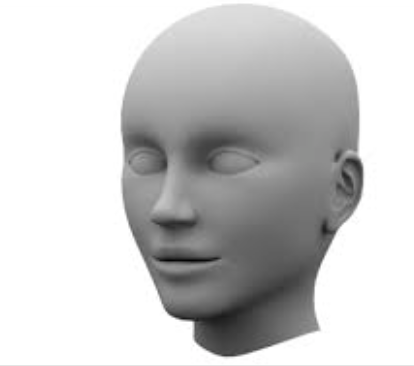
\includegraphics[width=0.3\textwidth]{head.png}
%	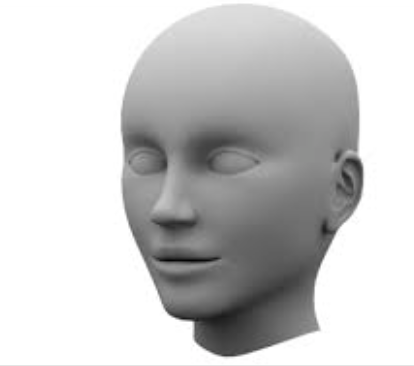
\includegraphics[width=0.3\textwidth]{head.png}
%	\caption{Frames from basic system preview}
%\end{figure}

As mentioned, the basic system only took one axis into account and so only altered the "Roll" Euler angle. This system although simple, showed promising results and provided the workflow to have a working system that synthesised head motions, saved them into a .head file containing the Euler angle change for each frame which can be read in by the PoserPython script and assigned to character to be rendered out.

\section{Random System}

Low correlation NOT no correlation.\\
Describe what value used. \\ between (0 \&100)\\
For each axis (half scaling for non nods)\\

The basic system itself produced a natural nodding motion, but after having compared the output of the basic system with the motion recordings, especially comparing different individuals speaking the same sentence there didn't seem to be any kind of correlation between what the participants were saying and how their head movements changed. To represent this finding the second system moved away from trigonometric functions.

\subsection{Discrete Head Motions}

The next system was designed to assign random discrete numbers to each word in the utterance for all Euler angles and apply a form of smoothing to make the random assignment seem smooth and natural even though it was completely random. 

\subsection{Smoothing}

To synthesise smooth head motions between random points multiple interpolation algorithms were considered. Spherical Linear Interpolation (Slerp) was the first that was considered and was already used in similar research \cite{rigid_head_motion}. There was difficulty when trying to implement Slerp due to the choosing Euler angles as the unit of rotation. Euler angles are difficult to apply interpolation \cite{quartionions}, Slerp commonly uses Quartinions which are more complex. Another method of interpolation which was derived from Slerp which was considered was the Bezier Interpolation algorithm, invented by Pierre Bezier a french mathematician was much simpler to implement than Slerp.

A recursive Bezier function was implemented which, given a list of points return a formula representing the a smooth interpolation between said points. Unlike Slerp, Bezier's smoothing algorithm doesn't take the interpolated line to the given points which works well given this scenario. It helped to smooth out the randomness and generate natural motions. (Figure 4.5)

EXPLAIN BEZIER PARAMETERS \\

\begin{figure}
	$$ B(t) = \sum_{i=0}^n {n \choose i} (1-t) t^i P^i $$ THIS IS BAD FIX IT\\
	\caption{Recursive Bezier Definition} 
\end{figure}

The random system calculated a Bezier function for each of the Euler angles and returned a dictionary containing the Euler angle change for each frame of the animation which was passed to output.py.

%\begin{figure}
%	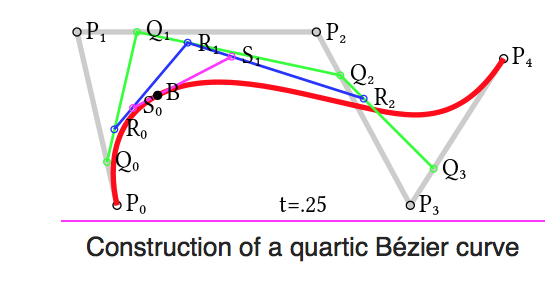
\includegraphics[width=0.7\textwidth]{bezier_example.png}
%	\caption{Example of Bezier}
%\end{figure}

\begin{figure}
	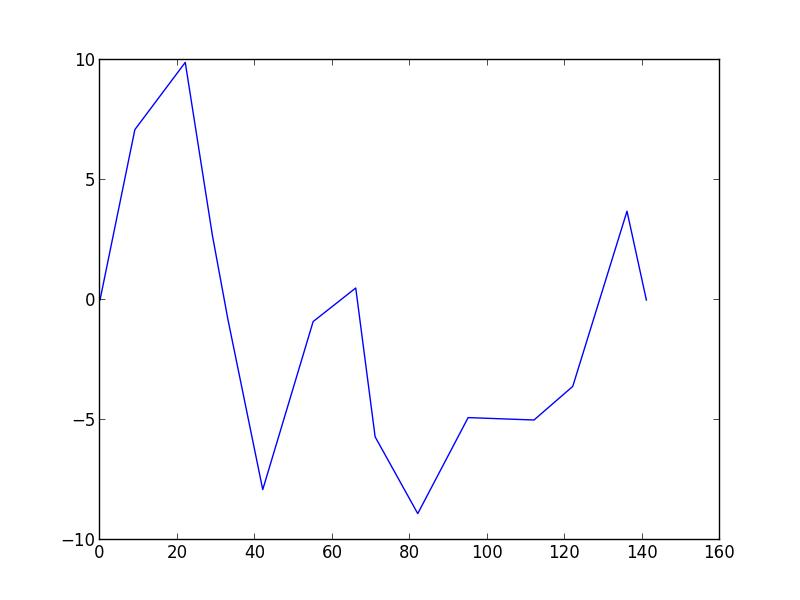
\includegraphics[width=.5\textwidth]{figure_1.png}
	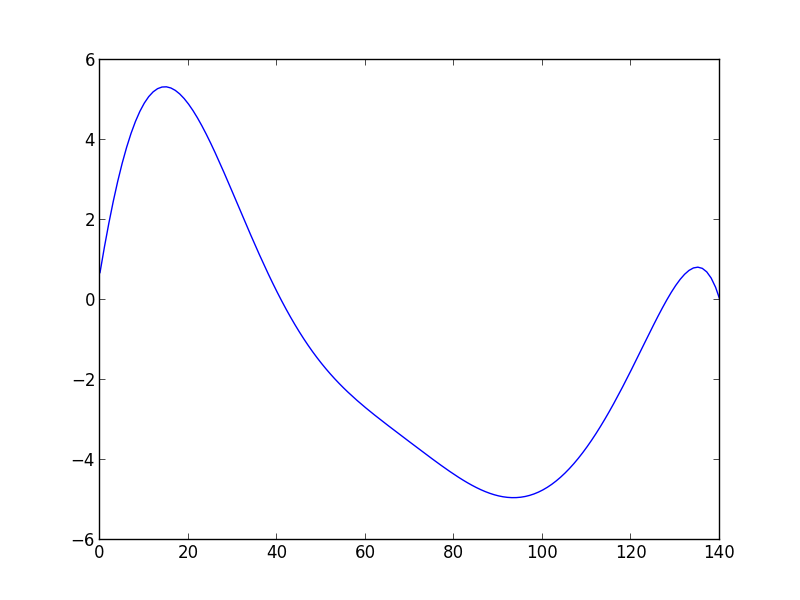
\includegraphics[width=.5\textwidth]{figure_2.png}
	\caption{Applying Bezier Smoothing to the discrete points}
\end{figure}

\subsection{Introduction of noise}

The output of the second system when mapped to a character in poser showed promise, the motions were smooth and looked like they could have been recorded from actual participants, however the motions produced were deemed too smooth and approached the uncanny valley, looking unnatural.

To counteract this issue a probability based assignment was introduced which adds or subtracts a very small percentage with the purpose of adding noise to the output. This reduced the feeling of the uncanny valley and lead to good initial results.

UNIFORM OR GAUSSIAN \\
WHAT VALUES USED \\

%\begin{figure}
%	\centering
%	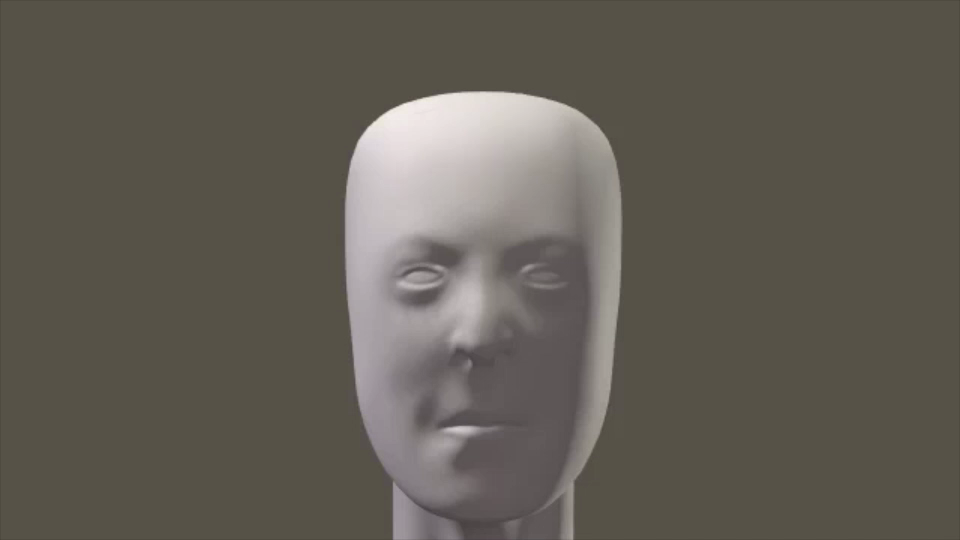
\includegraphics[width=.3\textwidth]{fightclub1.png}
%	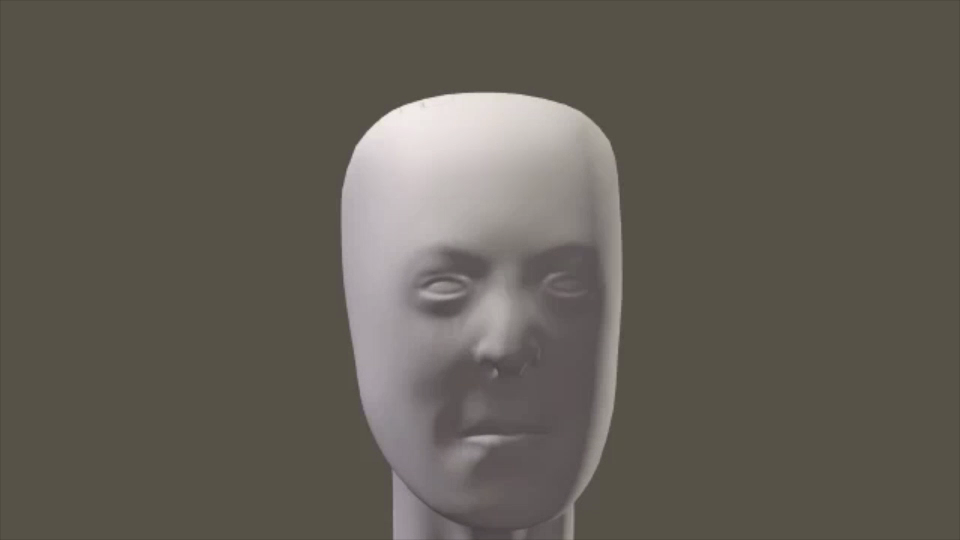
\includegraphics[width=.3\textwidth]{fightclub3.png}
%	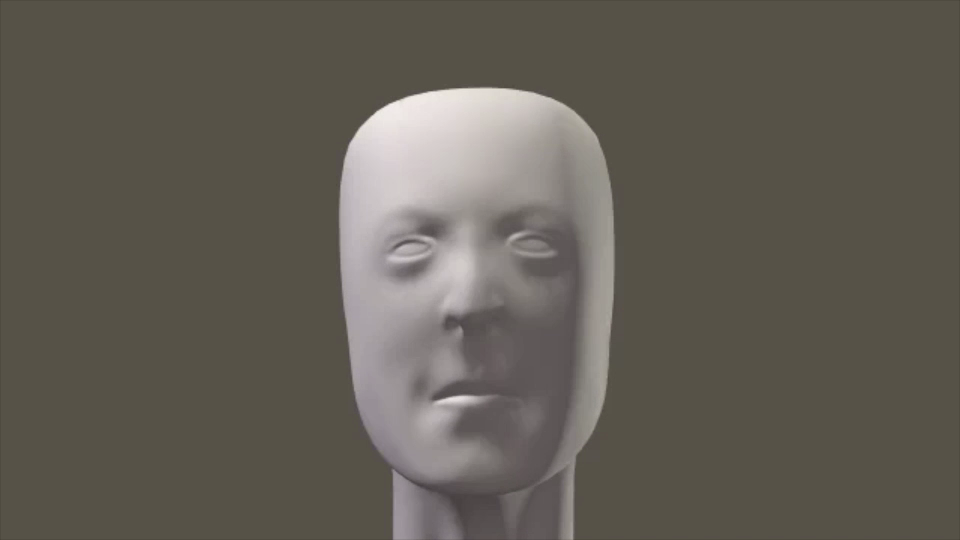
\includegraphics[width=.3\textwidth]{fightclub4.png}
%	\caption{Frames from the random system visualisation}
%\end{figure}

\section{Rule-Based System}

The Rule-Based system uses the output from Festival to apply manually written rules in order to synthesise head motions. Having considered the initial results of the previous two system the third built upon those ideas integrating with the rules derived from the multiple hypotheses outlined in chapter 3.

As there if not a 1 to 1 mappings between head motions and the words found in speech, the rule-based system removes stop words : words that are very common or are short function words like 'the', 'and' and 'which'. The system used the list of stop words from the NLTK library.

\subsection{Using the information from festival}

\subsection{Parametric Smoothing}
%- Felt Bezier did not look like natural head motions \\
%- Comparison with data looked too smooth even with noise \\
%- Moved towards First Order equations \\
%- commonly used in electronics \\
%- felt it aligned with recorded head motions more\\

One of the drawbacks from the initial reviews of the random system was that Bezier smoothing does not look like natural head motions. Having compared the output from the random system to the data recordings, the videos seemed to be more sharp and discontinuous, initially while smoothing out toward the end of the motion. The observed effect was similar to that of a first order differential equation, commonly used in electronics to represent the power in a circuit. Rising very quickly to begin with but slowing and smoothing off before reaching the desire level of output. 

\begin{figure}
	\centering
	$$ Y = K.A * (1 - e^{\sfrac{-t}{T}})$$
	\\
	%K.A = Steady State Gain\\
	%T = Time Constant\\
	%t = time\\
	
	\caption{First Order Equation Definition} 
\end{figure}

% ============================================================= %
\chapter{Evaluation}

To evaluate the Text-Driven Head Motion System I performed both subjective analysis and objective analysis. The aim for the project was to develop a system which generates life-like talking heads with head motions that seem realistic and natural so it was important for humans to evaluate if the head motions were natural or not. Having a unit of measurement describing how close to the original head motions was also necessary in evaluating the system.

\section{Subjective Analysis}

\subsection{Design Overview}

The evaluation system was designed with many factors taken into account. To effectively isolate the head motions for evaluations and make sure that participants were not affected or influenced by other factors, care was taken to ensure that as much as possible would remain constant, only changing the head motions.

Volunteers were shown 5 different video clips and were asked to evaluate how natural they felt the head motions were. Of the 5 videos, 3 were synthesised from the Text Driven Talking Heads system and 2 videos were taken from real recordings. Participants were not told anything about the videos and so did not know if the videos were synthesised or real. This was to eliminate any potential bias that could be introduced by telling the participants some of the videos were real and some were not and made sure that the participants focused on the task.

It was important for participants to be able to review their evaluation and update their choices as their subjective idea of what natural head motions are could easily change after watching the videos. Participants were encouraged to watch the videos more than once and update their evaluation are necessary until they were content with their evaluation.

\subsection{Implementation}

The evaluation platform was implemented in a web-based format using HTML5, Python and Flask \cite{flask}, a Python framework used for web development. The website (shown in figure 5.1), showed the 5 videos side by side with sliders allowing the users to click and drag the slider to a level they felt reflected how natural the video above that slider was. This approach accomplished two things: having sliders ranging from 0 to 100 allowed for much greater precision than asking participants to rate the video from 1-5 or 1-10 and also helped users generate numeric feedback without the need to arbitrarily assign a numerical value.

As outlined in the design overview, only once participants were content with their evaluation would the results be recorded. The 'submit' button commits the users evaluation to a text file. This was suitable for the purpose of the evaluation system as it very simple to implement and had little development overhead.

\begin{figure}
	\centering
	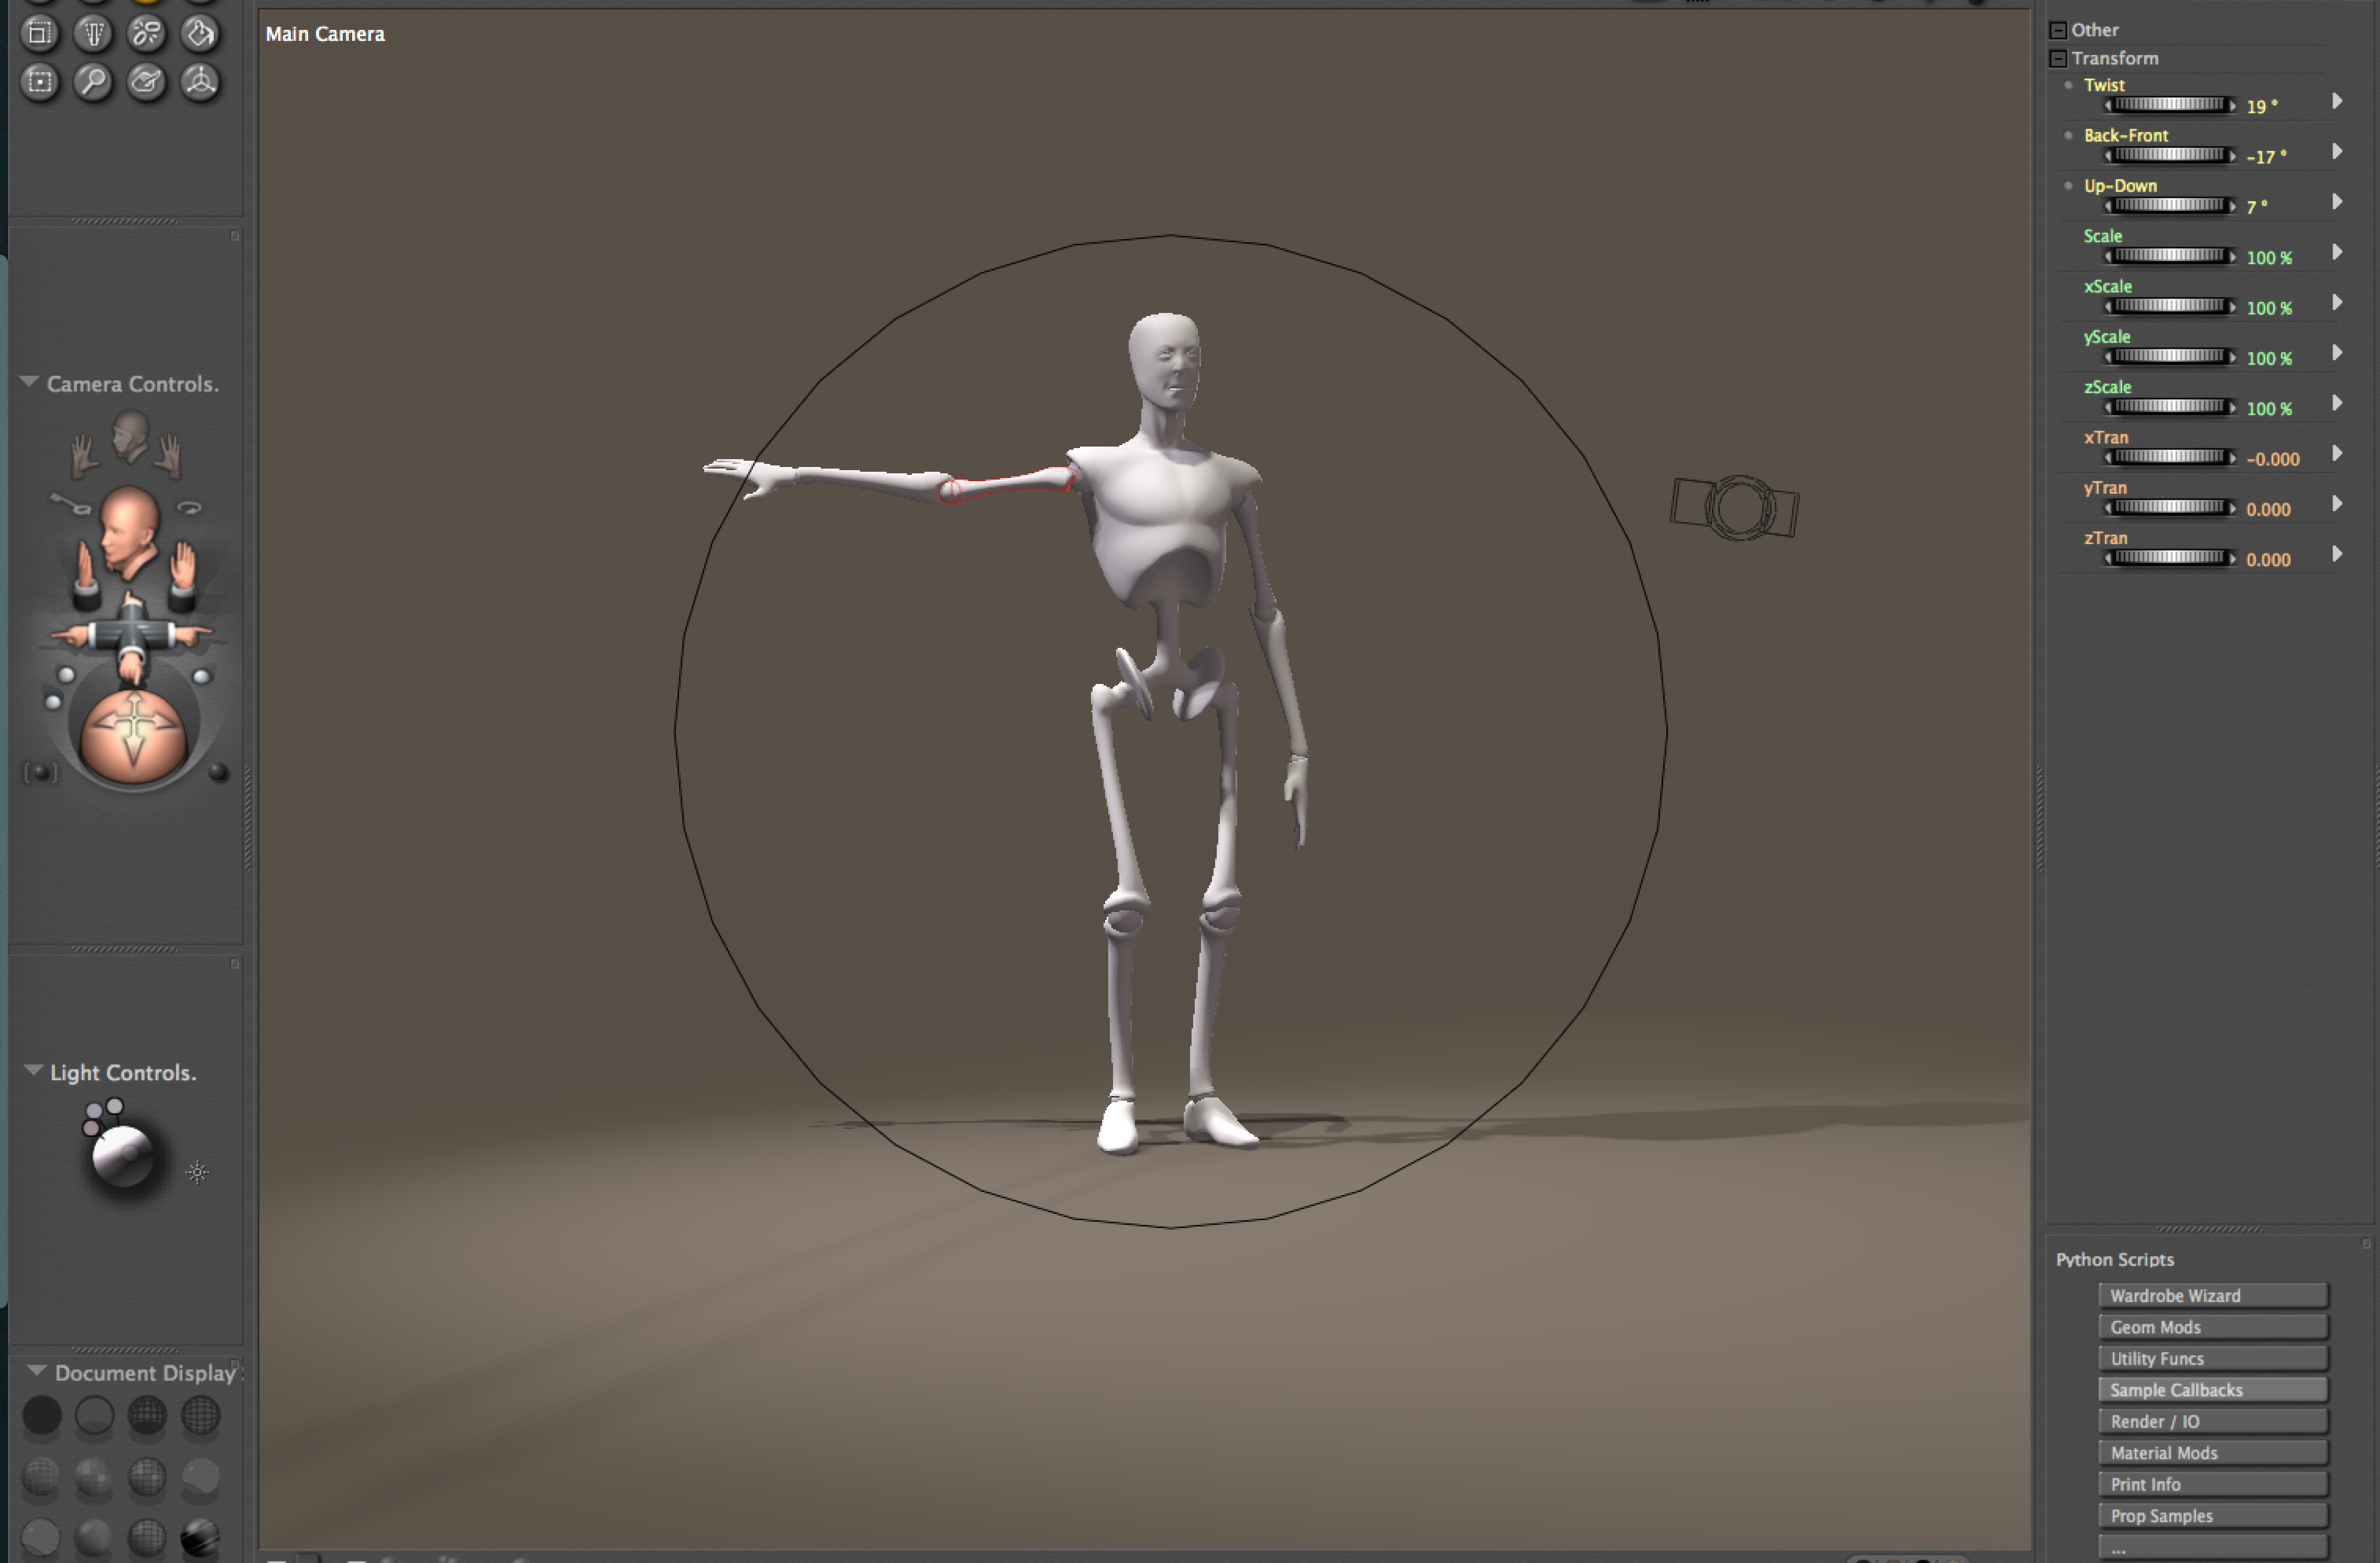
\includegraphics[width=.7\textwidth]{poser.png}
	\caption{Evaluation Platform}
\end{figure}

\subsection{Preliminary Results and feedback}

Preliminary evaluations were carried out to to test the evaluation platform. A small number of volunteers were asked to perform the evaluation and were asked a series of questions about the environment.

\begin{enumerate}
\item{How difficult was the task? What were the areas of difficulty?}
\item{Did you find the 3D avatars creepy?}
\item{Would the task be easier or more diffuclt with longer videos?}
\end{enumerate}

This was to try and improve the user experience before the final evaluation. The questions chosen were to address some key concerns regarding the environment. The participants were to feel comfortable during the evaluation process and if they videos they were evaluating were in the uncanny valley, many participants would feel discomfort which could negatively impact results. Gauging if participants felt the videos were too short or too long was important as well, the video needed to be of appropriate length so users had the right amount of information to effectively evaluate the videos.

\begin{quotation}
"Everything was fairly easy." - Participant 1

"Another quote" - Participant 2
\end{quotation}

\subsection{Results}

- Taken on  board suggestions from preliminary feedback \\
- 15 volunteers \\
- Good results for Random system \\
- Good results for rule-based system \\
- Bad results for ones taken from data \\

\subsection{Conclusions}

\section{Objective Analysis}

- Calculate difference in Euler angles\\
- Compare each system to two recordings due to lack of transcriptions\\

\subsection{Results}
% ============================================================= %
\chapter{Conclusions}

\section{System Overview}

\section{Discussion}

\subsection{Classification and Regression Trees}

\subsection{Data Driven System}

\section{Future Work}

\subsection{Expansion of techniques}

\subsection{Second Order Smoothing}
	
\bibliographystyle{plain}
\bibliography{diss}

\end{document}
